
%%%%%%%%%%%%%%%%%%%%%%%%%%%%%%%%%%%%%%%%%%%%%%%%%%%%%%%%%%%%%%%%%%%%%%%%
%    Option test file, will be created during the first LaTeX run:
\begin{filecontents}{exercise.thm}
\def\th@exercise{%
  \normalfont % body font
  \thm@headpunct{:}%
}
\end{filecontents}
%%%%%%%%%%%%%%%%%%%%%%%%%%%%%%%%%%%%%%%%%%%%%%%%%%%%%%%%%%%%%%%%%%%%%%%%

\documentclass[12pt,openright,oneside,a4paper,english,french,spanish,brazil]{article}
% ---
% Pacotes básicos 
% ---
\usepackage{lmodern}			  % Usa a fonte Latin Modern			
\usepackage[T1]{fontenc}		  % Selecao de codigos de fonte.
\usepackage[utf8]{inputenc}	      % Codificacao do documento (conversão automática dos acentos)
\usepackage[top=20mm, bottom=20mm, left=20mm, right=20mm]{geometry}
\usepackage{lastpage}			  % Usado pela Ficha catalográfica
\usepackage{indentfirst}		  % Indenta o primeiro parágrafo de cada seção.
\usepackage{color}				  % Controle das cores
\usepackage{graphicx}			  % Inclusão de gráficos
\usepackage{microtype} 		      % para melhorias de justificação
\usepackage{booktabs}
\usepackage{multirow}
\usepackage[table]{xcolor}
\usepackage{subfig}
\usepackage{epstopdf}
\usepackage{hyperref}
\usepackage[mathcal]{eucal}
\usepackage{amsmath}               % great math stuff
\usepackage{amsfonts}              % for blackboard bold, etc
\usepackage{amsthm}                % better theorem environments
\usepackage{amssymb}
\usepackage{mathrsfs}
\DeclareMathAlphabet{\mathpzc}{OT1}{pzc}{m}{it}
\usepackage{undertilde}            % botar tilde embaixo da letra
\usepackage{mathptmx}          % fonte
\usepackage{latexsym}
\usepackage{makeidx}            % para definir o índice
\usepackage{epsfig}             % para introduzir figuras no formato eps
\usepackage{graphicx,color}     % permite a inclusao de figuras
\usepackage{verbatim}
\usepackage{gensymb}
\usepackage{titling}
\newcommand{\subtitle}[1]{%
	\posttitle{%
		\par\end{center}
	\begin{center}\Large#1\end{center}
	\vskip0.5em}%
}
\newtheorem{df}{Definição}
\newtheorem{ex}{Exemplo}
\newtheorem{teo}{Teorema}

\newtheoremstyle{note}% name
  {3pt}%      Space above
  {3pt}%      Space below
  {}%         Body font
  {}%         Indent amount (empty = no indent, \parindent = para indent)
  {\itshape}% Thm head font
  {:}%        Punctuation after thm head
  {.5em}%     Space after thm head: " " = normal interword space;
        %       \newline = linebreak
  {}%         Thm head spec (can be left empty, meaning `normal')

\theoremstyle{note}
\newtheorem{note}{Note}

\newtheoremstyle{citing}% name
  {3pt}%      Space above, empty = `usual value'
  {3pt}%      Space below
  {\itshape}% Body font
  {}%         Indent amount (empty = no indent, \parindent = para indent)
  {\bfseries}% Thm head font
  {.}%        Punctuation after thm head
  {.5em}%     Space after thm head: " " = normal interword space;
        %       \newline = linebreak
  {\thmnote{#3}}% Thm head spec

\theoremstyle{citing}
\newtheorem*{varthm}{}% all text supplied in the note

\newtheoremstyle{break}% name
  {9pt}%      Space above, empty = `usual value'
  {9pt}%      Space below
  {\itshape}% Body font
  {}%         Indent amount (empty = no indent, \parindent = para indent)
  {\bfseries}% Thm head font
  {.}%        Punctuation after thm head
  {\newline}% Space after thm head: \newline = linebreak
  {}%         Thm head spec

\theoremstyle{break}
\newtheorem{bthm}{B-Theorem}

\theoremstyle{exercise}
\newtheorem{exer}{Exercise}

\swapnumbers
\theoremstyle{plain}
\newtheorem{thmsw}{Theorem}[section]
%\newtheorem{corsw}[thm]{Corollary}
\newtheorem{propsw}{Proposition}
%\newtheorem{lemsw}[thm]{Lemma}

%    Because the amsmath pkg is not used, we need to define a couple of
%    commands in more primitive terms.
\let\lvert=|\let\rvert=|
\newcommand{\Ric}{\mathop{\mathrm{Ric}}\nolimits}

%    Dispel annoying problem of slightly overlong lines:
\addtolength{\textwidth}{8pt}

\title{ \textbf{Notas de Aula}}
\subtitle{\textbf{Álgebra Linear}}
\author{\textbf{Fernando Contreras}\\
	\large Nucleo de Tecnologia\\
	Universidade Federal de Pernambuco (UFPE)}



\begin{document}
	\begin{center}
		Universidade Federal de Pernambuco (UFPE)\\
		Centro Acadêmico do Agreste\\
		Núcleo de Tecnologia\\
		
		Lista 3 de Álgebra Linear\\
		Prof. Fernando RL Contreras
	\end{center}


Sejam os seguintes problemas

\begin{itemize}
	\item[1.] Se $A$ é uma forma bilinear simétrica e $Q$ a forma quadratica associada a ela mostre que $A(v,w)=\frac{1}{4}Q(v+w)-\frac{1}{4}Q(v-w)$.\\
	Exer 10 pag. 282 Boldrini 
\end{itemize}
\begin{itemize}
	\item[2.] Seja $Q(x,y)=x^{2}+12xy-4y^{2}$. Determine uma base $\beta$ tal que: $[v_{\beta}=\begin{bmatrix}
	x_{1}  \\
	y_{1}  
	\end{bmatrix}$ e $Q(v)=ax_{1}^{2}+by_{1}^{2}$.
	 Exer 9, pag. 282 Boldrini
\end{itemize}

\begin{itemize}
	\item [3.] (a) Seja $A((x,y),(x^{'},y^{'}))=3xx^{'}+yy^{'}$. Ache a forma quadrática $Q:\mathbb{R}^{2}\longrightarrow \mathbb{R}$ associada a $A$.\\ (b) Seja $Q(x,y)=2x^{2}+4xy-y^{2}$. Ache a matriz da forma bilinear associada.\\ 
     Exer 8, pag. 282 Boldrini
\end{itemize}
\begin{itemize}
	\item[4.] (a) Seja $A:\mathbb{R}^{3}\times\mathbb{R}^{3} \longrightarrow \mathbb{R} $ definida por $A((x,y,z),(x^{'},y^{'},z^{'}))=xy^{'}+xz^{'}-yx^{'}-zy^{'}+zz^{'}$. Ache a matriz de $A$ em relação às bases $i)$ canônica $ii)$ $ \left\lbrace  (1,1,1), (1,1,0), (0,1,0) \right\rbrace $.\\
	(b) $A:\mathbb{R}^{2}\times\mathbb{R}^{2} \longrightarrow \mathbb{R} $ definida por  $A((x,y),(x^{'},y^{'}))=xy^{'}-yx^{'}$ e $\alpha= \left\lbrace  (1,1), (-1,1) \right\rbrace $. Ache $[A]_{\alpha}^{\alpha}$.\\
 Exer 6, pag. 281 Boldrini
\end{itemize}
\begin{itemize}
	\item[5.] Verifique se as aplicações abaixo são formas bilineares.\\
	(a) $F:\mathbb{R}^{2}\times\mathbb{R}^{2} \longrightarrow \mathbb{R} $. Definida por $F((x_{1},y_{1}),(x_{2},y_{2}))=x_{1}+y_{2}$.\\
	(b) $G:V\times V \longrightarrow \mathbb{R} $ definida por $G(u,v)=\left\langle u,v \right\rangle $\\
 Exer 2, pag. 281 Boldrini	
\end{itemize}

\begin{itemize}
	\item[6.] Uma forma bilinear $f$ sobre $\mathbb{R}^{3}$ esta caracterizada pela matriz $A=\begin{bmatrix}
	1    & 2 & -1  \\
	1    & 0 & -2 \\
	0    & 1 & 1 
	\end{bmatrix}$.\\
	 $i)$ Obter $f(u,v)$.\\
	  $ii)$ Determinar a matriz de $f$ com respeito da base $ \left\lbrace (1,1,1), (1,1,0), (1,0,0) \right\rbrace $.\\ 
 Exer 9-17, pag. 321 Armando Rojo		
\end{itemize}
\begin{itemize}
	\item[7.] Seja a forma bilinear $f(u,v)=ax_{1}y_{1}+cx_{1}y_{2}+cx_{2}y_{2}$. Que condições devem satisfazer $a$, $b$ e $c$ para que:\\
	(a) $f(u,v)=f(v,u)$ para todo $u,v, \in \mathbb{R}^{2}$.\\
	(b) $f(u,v)=-f(v,u)$ para todo $u,v, \in \mathbb{R}^{2}$. \\
 Exer 8, pag. 215 Caliolli		
\end{itemize}
\begin{itemize}
	\item[8.] Identifique a figura.\\
	(a).\quad $3x^{2}+2y^{2}+3z^{2}+2xz=2$\\
	(b).\quad $y^{2}+2z^{2}+2\sqrt{3}yz=0$\\
	(c).\quad $3x^{2}+2xy+3y^{2}-\sqrt{2}x=0$\\
	(d).\quad $3x^{2}-4\sqrt{3}xy-y^{2}+20y-25=0$ \\
	 Exer 11.6, pag. 305 Boldrini
\end{itemize}
\begin{itemize}
	\item[9.] Identifique a figura e ache sua posição (esboçar) quando a sua equação é:\\
	 (a).\quad $-5y^{2}+2xy-8xz+2yz=0$\\
	 (b).\quad$x^{2}+xy+y^{2}-3=0$\\
	 (c).\quad$9x^{2}+16y^{2}+25z^{2}+24xy-40x+30y=0$\\
	 (d).\quad$xy+x+y=0$\\
	 Exer 11.6, pag. 305 Boldrini
\end{itemize}
\begin{itemize}
	\item[10.] Dê a solução do sistema lineares:\\
	(a) $\begin{cases}
	\frac{dx}{dt}=-9x+19y+4z,\\
	\frac{dy}{dt}=-3x+7y+z,\\
	\frac{dz}{dt}=-7x+17y+2z
	\end{cases}$\\
	(b) $\begin{cases}
	\frac{dx}{dt}=4x-3y,\\
	\frac{dy}{dt}=5x-4y
	\end{cases}$ com condição inicial $x(0)=1$, $y(0)=2$\\
	(c)$\begin{cases}
	\frac{dx}{dt}=x+y,\\
	\frac{dy}{dt}=-x+3y
	\end{cases}$\\
	(d)$\begin{cases}
	\frac{dx}{dt}=-5x,\\
	\frac{dy}{dt}=-5y
	\end{cases}$ com condição inicial $x(0)=1$, $y(0)=2$\\
		 Exer xxx, pag. 329 Boldrini
\end{itemize}
\begin{itemize}
	\item[11.] Num circuito LC, seja um indutor de indutância $L$ ligado em série com um capacitor de capacitância $C$. Seja $i$ a corrente que circula no circuito e $q$ a carga no capacitor.\\
	\begin{figure}[!h]
		\begin{center}		
			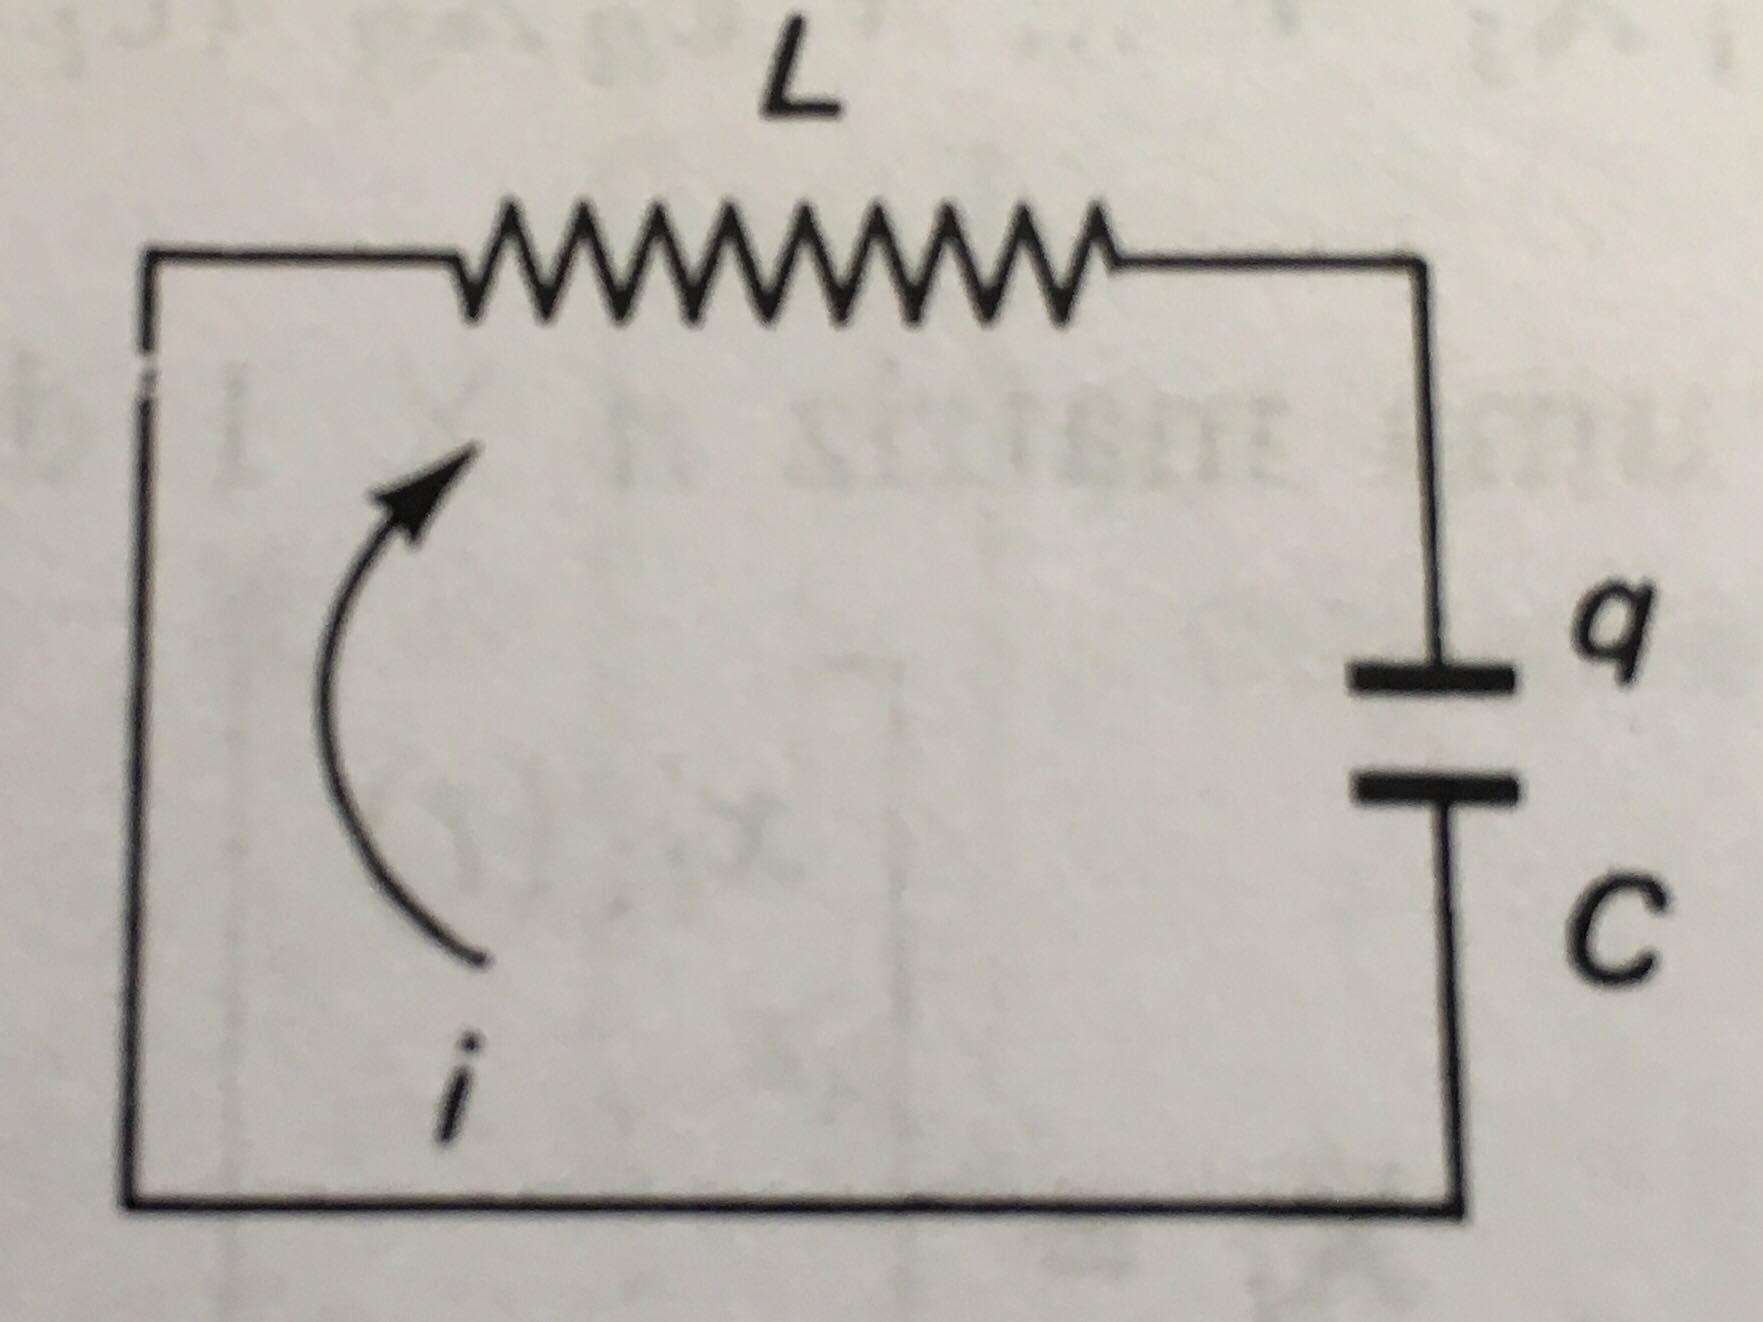
\includegraphics[width=0.3\linewidth,angle=0]{Figura1.jpg}
		\end{center}
	\end{figure}\\
    Suponhamos incialmente, que a corrente no circuito seja $i_{o}$ e o capacitor tenha carga $q_{o}$. sabendo que a diferença de potencial no indutor é $L\frac{di}{dt}$ e no capacitor $\frac{q}{C}$, temos o sistema de equações diferencias\\
    $\begin{cases}
    L\frac{di}{dt}+\frac{q}{C}=0,\\
    \frac{dq}{dt}=i
    \end{cases}$\\	
	Encontre as expressões de carga e da corrente em função do tempo.\\
		 Exer 6, pag. 330 Boldrini
\end{itemize}
\begin{itemize}
	\item [12.]  Uma colonia de bactérias cresce a uma razão diretamente proporcional ao número de bactérias presentes. (Se chamarmos de $B(t)$ a quantidade de bactérias depois de um tempo $t$, isto significa que $\frac{d}{dt}B(t)=kB(t)$, $k=constante$.) Se o número de bactérias triplica em duas horas, quanto tempo será necessário para que tenhamos cinquenta vezes a quantidade inicial ?\\
	 Exer 1, pag. 329 Boldrini
\end{itemize}
\end{document}
